\documentclass[a4paper,12pt]{article}

%-------------------------------------------------------------------------------

\usepackage[final]{nips_2017}
\usepackage[utf8]{inputenc}

\usepackage{hyperref}
\usepackage{url}

\usepackage{amsmath}
\usepackage{amsthm}
\usepackage{amssymb}
\usepackage{amsfonts}

\usepackage{microtype}

\usepackage{graphicx}
\usepackage{tikz}

\usepackage{fullpage}

%-------------------------------------------------------------------------------

% \hypersetup{
%     colorlinks=true,
%     linkcolor=red,
%     filecolor=magenta,
%     urlcolor=cyan
% }

\DeclareMathOperator{\rmse}{RMSE}
\DeclareMathOperator{\nasa}{S}

%-------------------------------------------------------------------------------

\title{Prognostic Health Management for Turbofan Engines Using Deep Learning}

\author{
Aditya Gulati\\
\texttt{adgulati@stanford.edu} \\
\And
Jeetsagar Ghorai \\
\texttt{jghorai@stanford.edu} \\
}

%-------------------------------------------------------------------------------
\begin{document}

\begin{center}

\includegraphics[width=3cm, height=0.7cm]{CS230}
\end{center}
\maketitle

%-------------------------------------------------------------------------------

\section{Introduction}

Prognostic Health Management (\emph{PHM}) is a unified framework for
forecasting system health and reliability. Most systems of interest are
composed of multiple components. Failure of a component in a system can result
in adverse outcomes such as stoppage of operation, destruction of the system or
loss of life. In most cases, the failure of a component results from the
degradation of said component over the course of operation. Prognostic Health
Management is concerned with forecasting potential failures of systems by
monitoring the status of the components and the performance of the system.\(^{[1]}\) PHM
is an active area of research in reliability engineering and PHM techniques have
been applied to a variety of systems such as hydraulic pumps, Lithium ion
batteries, MOSFETs etc.

In most problems of interest, the data is available in the form of a time series
of sensor readings. Given this time series data, the aim of PHM is to predict
the Remaining Useful Life (\emph{RUL}) of the system. Predicting the potential
failure of a component allows the operator to plan for repair or replacement,
mitigate downtime and ensure the safety of the equipment and the environment.
Overestimating RUL leads to an unplanned failure, whereas underestimating RUL
leads to underutilization of the component.

%-------------------------------------------------------------------------------

\section{Dataset}

The aim of our work is to develop a prognostics model for turbofan aircraft
engines using deep learning. We have used the
\href{https://ti.arc.nasa.gov/tech/dash/groups/pcoe/prognostic-data-repository}
{Turbofan Engine Degradation Simulation Data Set-2} published by the Prognostics
Center of Excellence at NASA. This dataset contains run-to-failure trajectories
of a number of turbofan aircraft engines.\(^{[3]}\)

The published repository contains multiple datasets. One representative dataset,
\texttt{DS02}, consists of run-to-failure simulation data for nine engines.
In this dataset, the operating conditions are described using 4 attributes.
The model outputs the values of 14 measured physical properties and the
readings from 14 virtual sensors. Together, there are 32 features at every
time-step. In the dataset, the different engines are referred to as units. The
units with $u = 2, 5, 10, 16, 18, 20$ are the six training units and the units
with $u = 11, 14, 15$ are the three test units. The dataset is described in Figure1 and Figure2.

\begin{figure}
    \centering
    
\includegraphics[width=\linewidth]{flight_profile.png}
    \caption{How the altitude, Mach number, throttle-resolver angle and temperature at fan inlet changes throughout a single flight of unit 20}
    \label{fig:flight_profile}
\end{figure}


\begin{figure}
    \centering
    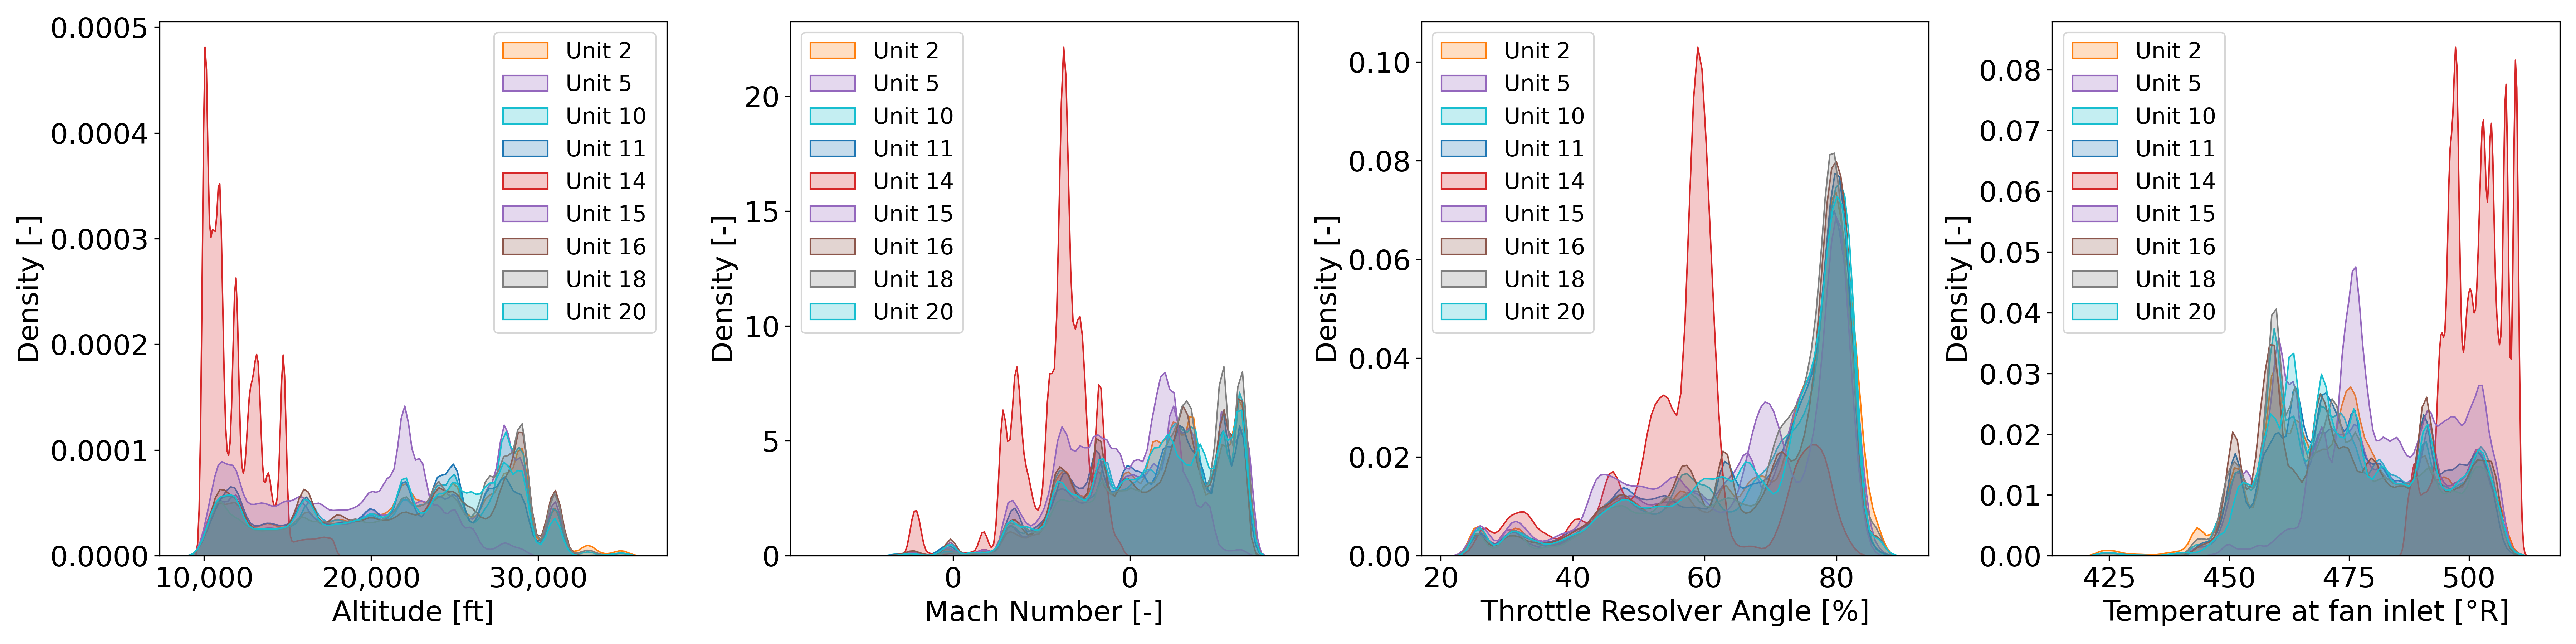
\includegraphics[width=\linewidth]{kde.png}
    \caption{Kernel density estimations of altitude, Mach number, throttle resolver angle and temperature at fan inlet for 6 training and 3 test units. The flight characteristics of units 14 and 15 are different from those of the training units.}
    \label{fig:unit_kde}
\end{figure}

%-------------------------------------------------------------------------------

\section{Problem Statement}

The dataset consists of the run-to-failure trajectories of $M+N$ units. There
are $s$ parameters which denote the operating condition of the aircraft and the
output of $p$ sensors are monitored at each time-step.

Suppose that the unit $i$ was operated for $m_i$ time-steps. The sensor
readings at time-step $t$ is denoted by $x_{i}^{(t)} \in \mathbb{R}^{p}$ and the
operating condition at time-step $t$ is denoted by
$w_{i}^{(t)} \in \mathbb{R}^{s}$. The RUL at time-step $t$ is denoted by
$y_{i}^{t} \in \mathbb{R}$.

Suppose that $X_i = \lbrack x_{i}^{(1)}, \ldots, x_{i}^{(m_i)} \rbrack^{T}$,
$W_i = \lbrack w_{i}^{(1)}, \ldots, w_{i}^{(m_i)} \rbrack^{T}$ and
$Y_i = \lbrack y_{i}^{1}, \ldots, y_{i}^{m_i} \rbrack^{T}$ Then,
$\mathcal{D}_{train} = \{W_i, X_i, Y_i\}_{i=1}^{N}$ constitutes the training
dataset and $\mathcal{D}_{test} = \{W_i, X_i, Y_i\}_{i=1}^{M}$ constitutes the
test dataset.

The aim of our project is to use $\mathcal{D}_{train}$ to train a deep learning
model $\mathcal{G}$ that predicts $\hat{Y}$, the RUL of the units in the
test dataset and minimizes some loss function $L$.

Suppose that the test unit $j$ is run for $m'_{j}$ time-steps and
$m = \sum_{j=1}^{M} m'_{j}$. Suppose that $\Delta^{(j)}$ is the difference
between the true RUL and the predicted RUL at time-step $j$, i.e.,
$\Delta^{(j)} = y^{(j)} - \hat{y}^{(j)}$. We have used two loss functions, the
root-mean-square error (RMSE) and NASA's scoring functions $\nasa$. These two
functions are defined as follows.

\[ \rmse = \sqrt{\frac{1}{m}\sum_{j=1}^{m}(\Delta^{(j)})^2} \]
\[ \nasa = \sum_{j=1}^{m}\alpha_{j}|\Delta^{(j)}| \mbox{ where, } \alpha_{j} = 
\left\{ \begin{array}{ll}
\frac{1}{13} & \mbox{ if } \Delta^{(j)} \geq 0 \\
\frac{1}{10} & \mbox{ if } \Delta^{(j)} < 0 \end{array} \right.\]

The coefficient $\alpha_{j}$ in NASA's scoring function is designed to
penalize over-estimation more than under-estimation.

\pagebreak

\section{Baseline : Deep Learning-Based Prognostics with Physics-Inferred Inputs}
The above turbo-engine dataset consists of operating conditions w, sensor measurements \(x_{s}\), virtual sensor measurements \(x_{v}\), model health parameters \(\theta\) as the input attributes and Remaining Useful Life (RUL) Y  as the target attribute.    
This work\(^{[4]}\) comprises of two different set of approaches to model the above regression problem data-driven model and UKF calibrated physics-based model.  Each of which is described as follows:
\subsection{Data-driven model}
In this approach we learn a mapping from enhanced input space \([w, x_{s}, x_{v},\theta]\) to RUL target Y using a 1-D CNN architecture. The CNN architecture is common for both the approaches and is shown in Figure 3. The enhanced input space in the dataset is obtained after using a simulation software N-CMAPPS which deviates from the real physics process of the turbofan engine. To mitigate this reality gap we present a calibration based approach in next subsection. 
\subsection{UKF calibrated physics-based model}
The sensor readings \(x_{s}, x_{v}\) and model health parameters \(\theta\) are obtained from a simulation software. This sensor consists of noise and is much deviated from the real world process. To counter this we use an Unscented Kalman Filter (UKF) as a tracking algorithm and induce the system physics. UKF tracking algorithm requires the current sensor readings and physics model as input along with some hyperparameters to drive the iterative process.
The above tracking algorithm provides us with a more accurate and correlated (physics enhanced) inputs \([\hat{x_{s}},\hat{x_{v}},\hat{\theta}]\) which are merged with operating conditions and sensor inputs \([w,x_{s}]\) . The result physics enhanced input space is \([w,x_{s},\hat{x_{s}},\hat{x_{v}},\hat{\theta}]\) which is mapped to target RUL Y using the same 1-D CNN. Detailed flow of this algorithm is given in description of Figure 3

\begin{figure}[h]
\centering
\includegraphics[scale=0.3]{FigAlgo1.png}
\caption{Figure borrowed from above paper\(^{[4]}\). Description: The non-linear system dynamical physics model is first approximated as  a FNN (trained offline), which is used as a system model in the UKF tracking algorithm, UKF further results in the physics enhanced input space which is merged with the simulation input space resulting  \([w,x_{s},\hat{x_{s}},\hat{x_{v}},\hat{\theta}]\) as the final physics-enhanced input. This is then sent into a 1-D CNN as shown in the right part of the figure above.}
\end{figure}

The physics-enhanced input consists of attributes \([w,x_{s},\hat{x_{s}},\hat{x_{v}},\hat{\theta}]\)  (total k attributes) for every last \(N_{tw}\) timestamps at a particular time t. Hence resulting in a 2-D \(k \times N_{tw}\) array (the convolution operation is shown in Figure 4). We use MSE as the loss function in the above 1-D CNN.

\begin{figure}[h]
\centering
\includegraphics[scale=0.3]{Conv.png}
\caption{Figure borrowed from above paper\(^{[4]}\), 1-D Convultion operation with stride in time-direction}
\end{figure}

\section{Baseline Results}
As described in the problem statement we use RMSE and NASA function as the evaluation metric for our algorithms, we have implemented the above two baseline approaches (from scratch), with taking units [2,5,10,16,18,20] as training units and [11,14,15] as testing units. 

\begin{table}[h]
\begin{center}
\begin{tabular}{ |c|c|c|c } 
 \hline
   & Data-driven Model &UKF Physics-based Model \\ 
  \hline
   RMSE & 7.662 & q \\ 
  \hline
   NASA-scoring function \( (s \times 10^{6})\) & 2.15 & s \\ 
  \hline
\end{tabular}
\caption{RMSE and NASA-scoring function evaluation on test-set for both algorithms}.
\end{center}
\end{table}
Both models are trained for 70 epochs with same CNN-architecture as shown in figure 3. For data-driven model, we have reported best results in  hyperparamer grid of Learning-rate [0.0001,0.001], \(N_{tw}\) [20,50] and batch size [256,512,1024] whereas in UKF physics model we are yet to perform hyperparameter tuning it is evaluated only at Learning rate - 0.0001, \(N_{tw}\) - 50 and batch size 512. We use adam optimisation with adagrad enabled in both approaches.

\section{Further course of action}

We would now like to explore the power of RNNs/LSTMs to model the temporal relation, the following CNN-RNN hybrid architecture in Figure 5 is borrowed from DeepSense\(^{[5]}\) paper. The main motivation here comes to the promising power of RNNs to model timeseries data which hasn't been modeled in the above existing approach. The input can be given similar to above and the expected outputs can be the RUL. This approach can be used for both data-driven dataset and UKF physics based dataset and will be compared with the benchmarks (baselines) given above.

\begin{figure}[h]
\centering
\includegraphics[scale=0.3]{FigAlgo2.png}
\caption{Figure Borrowed from DeepSense\(^{[5]}\) paper, the idea here is to send raw-sensor data as set of 2D arrays and expect RULs at output}
\end{figure}
The training strategy and loss function will be same as that of used in the previous approach.
If time permits, we also plan to put everything in a UI to give a better visualisation and illustration of how this system can be deployed in real-time.

\section*{References}

\medskip
\small
[1] Kwok L. Tsui, Nan Chen, Qiang Zhou, Yizhen Hai, Wenbin Wang, "Prognostics and Health Management: A Review on Data Driven Approaches", Mathematical Problems in Engineering, vol. 2015, Article ID 793161, 17 pages, 2015. https://doi.org/10.1155/2015/793161

[2] Biggio Luca, Kastanis Iason, "Prognostics and Health Management of Industrial Assets: Current Progress and Road Ahead", Frontiers in Artificial Intelligence,VOL 3, 2020, 88 pages, https://www.frontiersin.org/article/10.3389/frai.2020.578613, 10.3389/frai.2020.578613, 2624-8212   

[3] M. Chao, C.Kulkarni, K. Goebel and O. Fink (2021). "Aircraft Engine Run-to-Failure Dataset under real flight conditions", NASA Ames Prognostics Data Repository (http://ti.arc.nasa.gov/project/prognostic-data-repository), NASA Ames Research Center, Moffett Field, CA

[4] Chao, Manuel Arias et al. “Fusing Physics-based and Deep Learning Models for Prognostics.” ArXiv abs/2003.00732 (2020)

[5] Shuochao Yao and Shaohan Hu and Yiran Zhao and Aston Zhang and Tarek Abdelzaher, "DeepSense: A Unified Deep Learning Framework for Time-Series Mobile Sensing Data Processing", ArXiv abs/1611.01942




%-------------------------------------------------------------------------------


%-------------------------------------------------------------------------------
\end{document}
